\ifdefined\directlua
  \directlua{pdf.setminorversion(7)}    %% In case some pdf figures have higher versions.
\fi
\documentclass[letterpaper,10pt]{article}

\ifdefined\directlua
  \usepackage[style=numeric-comp,sorting=none,backref=true]{biblatex}
  \addbibresource{ref.bib}
\fi

\usepackage{graphicx}
\usepackage{amsmath}
\usepackage{amssymb}
%\usepackage{listings}

\ifdefined\directlua
  % Unicode fonts setup for lualatex/xelatex only
  \usepackage{unicode-math}
  \defaultfontfeatures{Scale=.92}
  \setmainfont{Lucida Bright OT}
  \setsansfont{Lucida Sans OT}
  \setmonofont{Lucida Sans Typewriter OT}
  \setmathfont{Lucida Bright Math OT}
  \setmathfont[version=bold]{Lucida Bright Math OT Demibold}
  \linespread{1.05}
\fi

\frenchspacing

\usepackage{microtype}
\usepackage{hyperref}

\DeclareMathOperator{\sort}{sorted}
\DeclareMathOperator{\Prob}{Prob}
\DeclareMathOperator{\Proj}{Proj}
\DeclareMathOperator{\ProjTAH}{Proj_{\text{TAH}}}
\DeclareMathOperator{\ProjSU}{Proj_{\text{SU}}}
\DeclareMathOperator{\OrdProd}{\prod_{\text{ord}}}
\DeclareMathOperator{\atan}{atan}
\DeclareMathOperator{\tr}{tr}
\DeclareMathOperator{\ReTr}{ReTr}
\DeclareMathOperator{\Herm}{H}
\DeclareMathOperator{\Real}{Re}
\DeclareMathOperator{\AHerm}{AH}
\DeclareMathOperator{\Arg}{Arg}
\newcommand{\ham}{\mathcal{H}}
\newcommand{\dd}{\mathop{\text{d}\!}}
\newcommand{\T}{\dag}
\newcommand{\J}{\mathcal{J}}
\newcommand{\X}{\mathcal{X}}
\newcommand{\n}{\mathcal{N}}
\newcommand{\g}{{\mathfrak{g}}}
\newcommand{\F}{\mathcal{F}}
\newcommand{\eU}{\mathbb{U}}
\newcommand{\eX}{\mathbb{X}}
\newcommand{\eN}{\mathbb{N}}
\newcommand{\Nc}{N_{\text{c}}}


\author{Xiao-Yong Jin for Lattice QCD ECP}
\date{\today}
\title{Field Transformation HMC}
\hypersetup{
 pdfauthor={Xiao-Yong Jin},
 pdftitle={Field Transformation HMC},
 pdfkeywords={Machine Learning, HMC, Ensemble, Lattice Gauge Theories},
 pdfsubject={Summary notes},
 pdflang={English}}

\begin{document}
\maketitle
\tableofcontents

\section*{Versions}
\label{sec:versions}

\begin{itemize}
\item April 20, 2021, version 0\\
Some text borrowed from the previous 1D XY model report.
\item June, 2021, version 1\\
Updated section~\ref{sec:gen-ft}.
\end{itemize}

\section{Introduction}
\label{sec:intro}
Following the arguments of ``Trivializing maps''~\cite{Luscher:2009eq},
to evaluate,
\begin{equation}
	⟨O⟩ = 1/Z ∫ \dd x O(x) e^{-S(x)},
\end{equation}
we perform a change of variable,
\begin{equation}
	x = F(y)
\end{equation}
with a vector functions $F$, we have
\begin{equation}
	⟨O⟩ = \frac{1}{Z} ∫ \dd y \left|\det[J(y)]\right| O\left(F(y)\right) e^{ -S\left(F(y)\right) },
\end{equation}
where the Jacobian matrix,
\begin{equation}
	J(y) = \frac{∂F(y)}{∂y}.
\end{equation}
$F$ has to satisfy,
\begin{itemize}
	\item Injective (1 to 1), from the new integration domain to the old.
	\item Continuously differentiable (or differentiable and have continuous inverse).
\end{itemize}

Rewrite the integral as,
\begin{equation}
	⟨O⟩ = \frac{1}{Z} ∫ \dd y O\left(F(y)\right) e^{ -S\left(F(y)\right) + \ln\left|\det[J(y)]\right| }.
\end{equation}
F is a trivializing map, when
\begin{equation}
	S(F(y)) - \ln\left|\det[J(y)]\right| = \text{constant}
\end{equation}
and our expectation value simplifies to
\begin{equation}
	⟨O⟩ = \frac{1}{Z} ∫ \dd y O\left(F(y)\right).
\end{equation}

In terms of HMC, we add the conjugate momenta, $π$,
and use the equations of motion derived from the Hamiltonian,
\begin{equation}
\label{eq:H}
	ℋ(y,π) = ½π² + S\left(F(y)\right) - \ln\left|\det[J(y)]\right|,
\end{equation}
as
\begin{align}
	\frac{\dd}{\dd t} π &= -\frac{∂}{∂y} ℋ = - J(y) S'\left(F(y)\right) + \tr\left[ J⁻¹ \frac{\dd}{\dd y}J \right], \\
	\frac{\dd}{\dd t} y &= \phantom{-}\frac{∂}{∂y} ℋ = π.
\end{align}
This is separable and can use the usual explicit, symplectic and symmetric
discrete integrators.

Consider a change of variable for $π$ and $y$,
\begin{align}
	π &= J(y) p = J\left(F⁻¹(x)\right) p, \\
	y &= F⁻¹(x),
\end{align}
with the Jacobian matrix of determinant $1$,
\begin{align}
	\J(p,x) &=
		\begin{bmatrix}
		J\left(F⁻¹(x)\right) & \frac{∂}{∂x} J\left(F⁻¹(x)\right) p \\
		0 & \frac{∂}{∂x} F⁻¹(x)
		\end{bmatrix}, \\
	\det[\J] &= 1.
\end{align}
We get a new Hamiltonian from equation~\eqref{eq:H},
\begin{equation}
	\tilde{ℋ}(x,p) = ½ p^† M p + S(x) - \ln\left|\det[J]\right|
\end{equation}
where the positive definite M,
\begin{equation}
	M(x) = J^†\left(F⁻¹(x)\right) J\left(F⁻¹(x)\right)
\end{equation}
is the kernel of the kinetic term considered
Duane et al~\cite{Duane:1986fy,Duane:1988vr}.


\section{Generalized field transformation \textcolor{magenta}{\textsc{updated}}}
\label{sec:gen-ft}
For a generic field transformation, we can take inspiration from an MD update, where
\begin{equation}
	U' ← U \exp[dt * \ProjTAH(M)].
\end{equation}
$U$ is covariant and $M$ (being sum of loops) is invariant under gauge transformation.

The most generic form of a field transformation could be
\begin{equation}
	U(x,μ)' ← \ProjSU \sum_L a_L \OrdProd[L(x,μ)],
\end{equation}
where $L(x,μ)$ is any line connecting gauge links from $x$ to $x+\hat{μ}$, $a_L$ is a scalar coefficient.
$L(x,μ)$ may or may not need to go through $U(x,μ)$.
wet may also have loops in it, and results in a polynomial of such loop after sum.

The $\ProjSU$ has to satisfy the constraint that
\begin{equation}
	X \ProjSU(M) Y = \ProjSU(X M Y)
\end{equation}
for any $X$ and $Y$ in the group.

We can, however, rewrite the equation to be similar to the MD update,
\begin{equation}
	U(x,μ)' ← \ProjSU \sum_L a_L U(x,μ) U(x,μ)^\dag \OrdProd[L(x,μ)],
\end{equation}
such that
\begin{equation}
	U(x,μ)^\dag \OrdProd[L(x,μ)]
\end{equation}
becomes a complete loop, which is gauge invariant.
We then have it in a simplified form,
\begin{equation}
	U' ← \ProjSU \sum_R a_R U R,
\end{equation}
where $R$ is any loop that start and stop at $x+\hat{μ}$.

We may write it in terms of
\begin{equation}
	U' ← \ProjSU \sum_{LR} a_{LR} L U R,
\end{equation}
such that L is any loop that start and stop at $x$, but since we can always pull the $U$ to the left by multiplying $U U^\dag$, the most generic form is simply,
\begin{equation}
	U' ← \ProjSU[ U (\sum_R a_R R) ],
\end{equation}
where $R$ is any loop that start and stop at $x+\hat{μ}$, and may or may not go through $U$.

We can multiply $U U^\dag$ again, so it becomes
\begin{equation}
	U' ← U { U^\dag \ProjSU[ U (\sum_R a_R R) ] }.
\end{equation}
If we had a $\ProjSU$ that satisfies
\begin{equation}
	X \ProjSU(M) Y = \ProjSU(X M Y)
\end{equation}
the above update would become
\begin{equation}
	U' ← U \ProjSU[ \sum_R a_R R ]
\end{equation}
though we need $\ProjSU$ satisfy a different constraint,
\begin{equation}
	X \ProjSU(M) X^\dag = \ProjSU(X M X^\dag)
\end{equation}
If we were allowed to do the above change of constraint to $\ProjSU$, it seems we could just use the projection in MD update,
\begin{equation}
	U' ← U \exp[ \ProjTAH( \sum_R a_R R ) ]
\end{equation}

It looks like we are only one step away from
\begin{equation}
	U' ← U \exp\left[ \frac{\dd}{\dd U} F( \ReTr A, \ReTr B, \ReTr C, ... ) \right]
\end{equation}
where $F$ is any analytical function or neural network, and $A$, $B$, $C$, ... are any closed
loops may or may not passing $U$.

We can simplify it by moving the $U$ independent loops out and keeping
the $U$ dependent loops simple,
\begin{equation}
\label{eq:gen-smear}
	U' ← U \exp\left[ c \atan\left[F(\ReTr X, \ReTr Y, ...)\right] \left[\frac{\dd}{\dd U} \ReTr[W]\right] \right]
\end{equation}
so that $F(\ReTr X, \ReTr Y, ...)$ only depends on $U$ independent loops,
while $W$ contains $U$ dependent loops, $c*\atan(F)$ is for restricting
the Jacobian to be positive definite, and $W$ is a sum of any loop
and its symmetrized versions including $U$.
The arbitrary function $F$ can take the form of a neural network.

For a transformation to be usable in HMC, we want a tractable Jacobian determinant.
One way to achieve this is updating gauge links in subsets,
such that each update to the subset of $U$ has a Jacobian matrix,
where the only nonzero entries are on its diagonal.


%\section{Test with 2D U(1) model without explicit neural networks}
%\label{sec:test-wo-nn}
%This test uses $F$ in equation~\eqref{eq:gen-smear} as a simple sum of similar loops,
specifically plaquettes and rectangles.

The loss function is
\begin{equation}
\label{eq:loss}
\begin{split}
	l(y',π'|y,π) &= - \frac{1}{N_{\text{batch}}} \sum_{\text{batch}}
	\max\left\{1, e^{H(y,π)-H(y',π')}\right\} \\
	&\Bigg(
		λ \frac{1}{N} \sum_x \left[ 1-\cos\left(P'ₓ-Pₓ\right) \right] \\
		&+ ρ \left[ \sum_x \sin(P'ₓ)-\sum_x \sin(Pₓ) \right]²
	\Bigg),
\end{split}
\end{equation}
where $(y',π')$ and $(y,π)$ are respectively the proposed and initial configuration
in the MD evolution,
$P_x = θ_{x,\hat{1}} + θ_{x+\hat{1},\hat{2}} - θ_{x+\hat{2},\hat{1}} - θ_{x,\hat{2}}$ is the plaquette phase at site $x$,
and the sum of $\sin$ is an approximate of the topological charge.
The test here uses $λ=0.1$ and $ρ=1.0$.

\begin{figure}
	\centering
	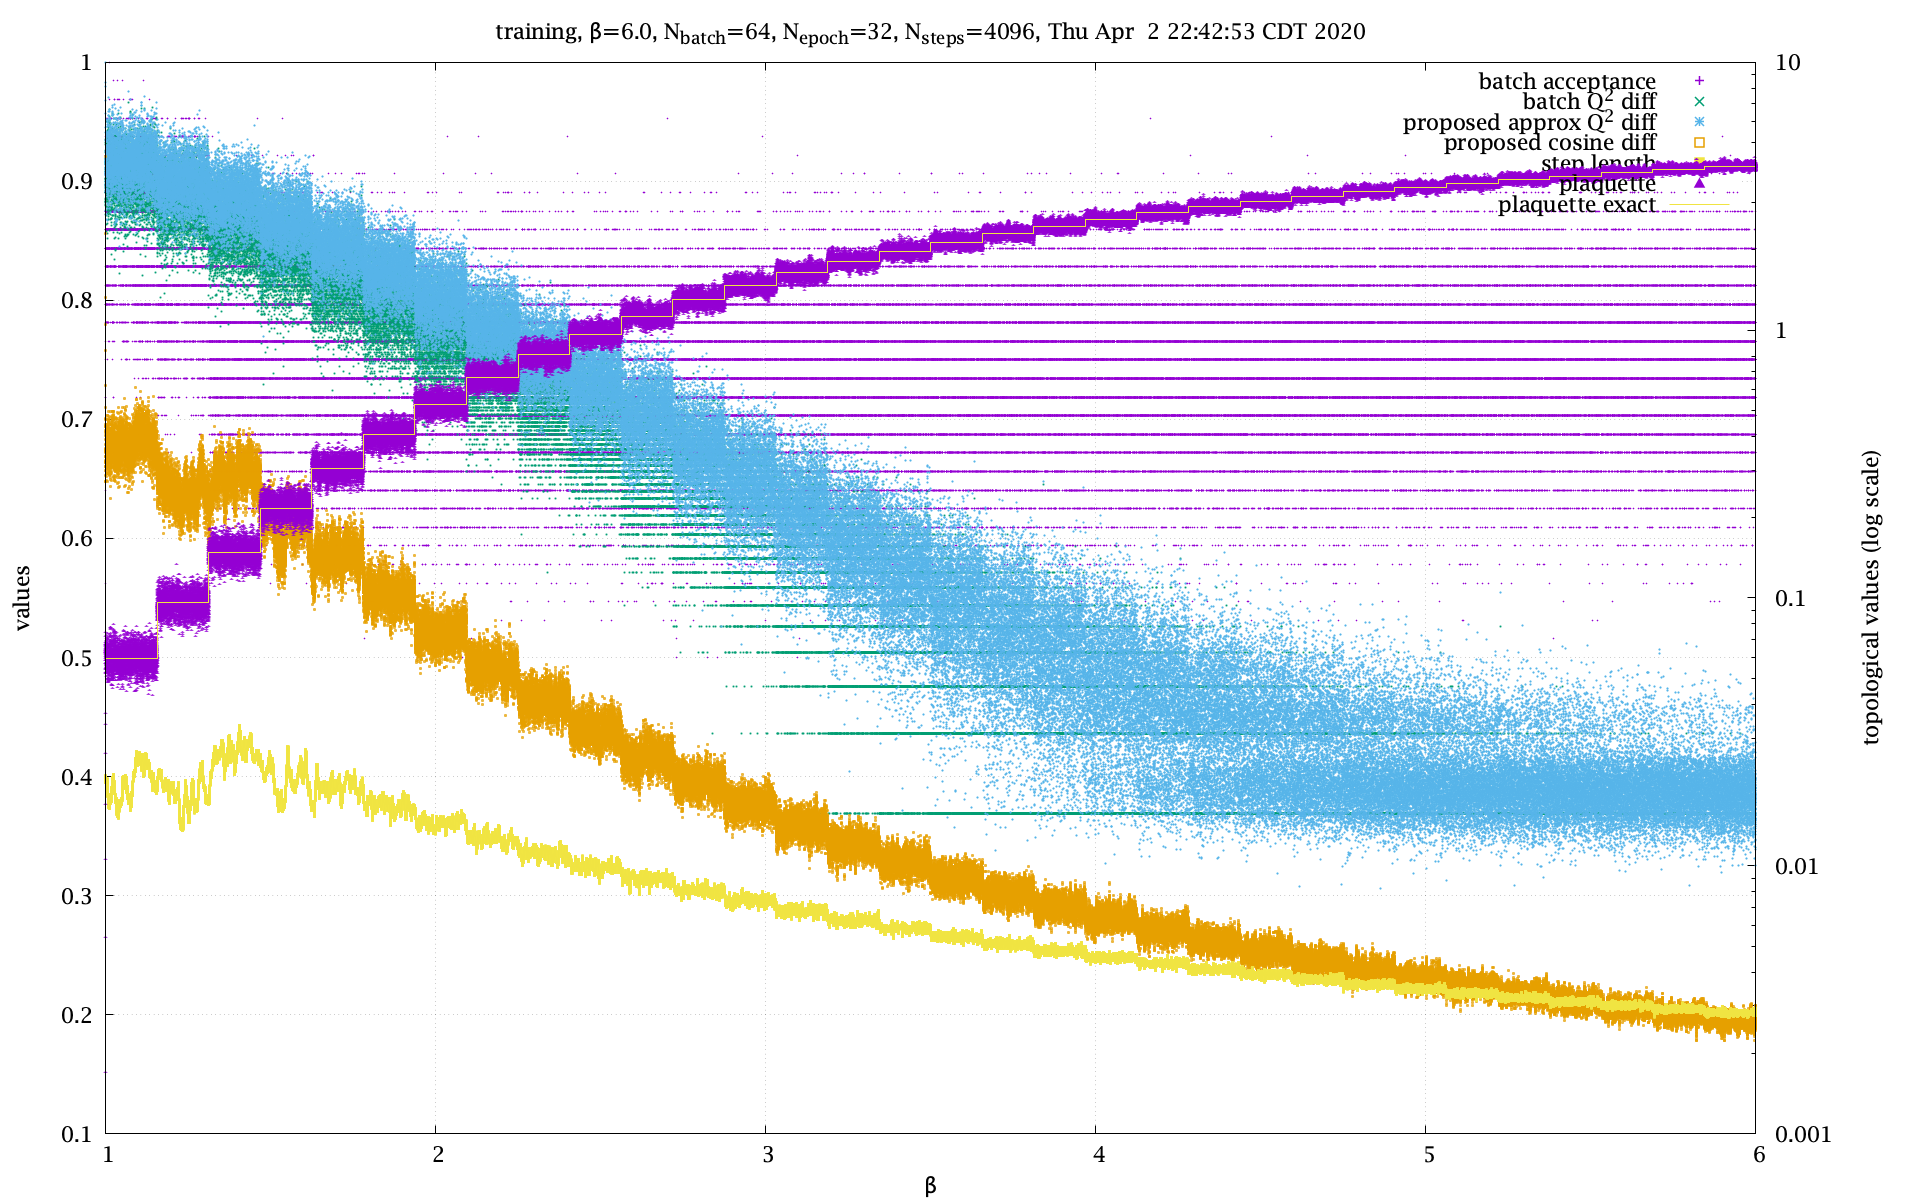
\includegraphics[width=\textwidth]{../../u1_2d/t4.png}
	\caption{\label{training-4}Annealed training steps for $V=8×8$ for HMC with 10 leapfrog steps,
	The only trainable parameter is the step size.}
\end{figure}

\begin{figure}
	\centering
	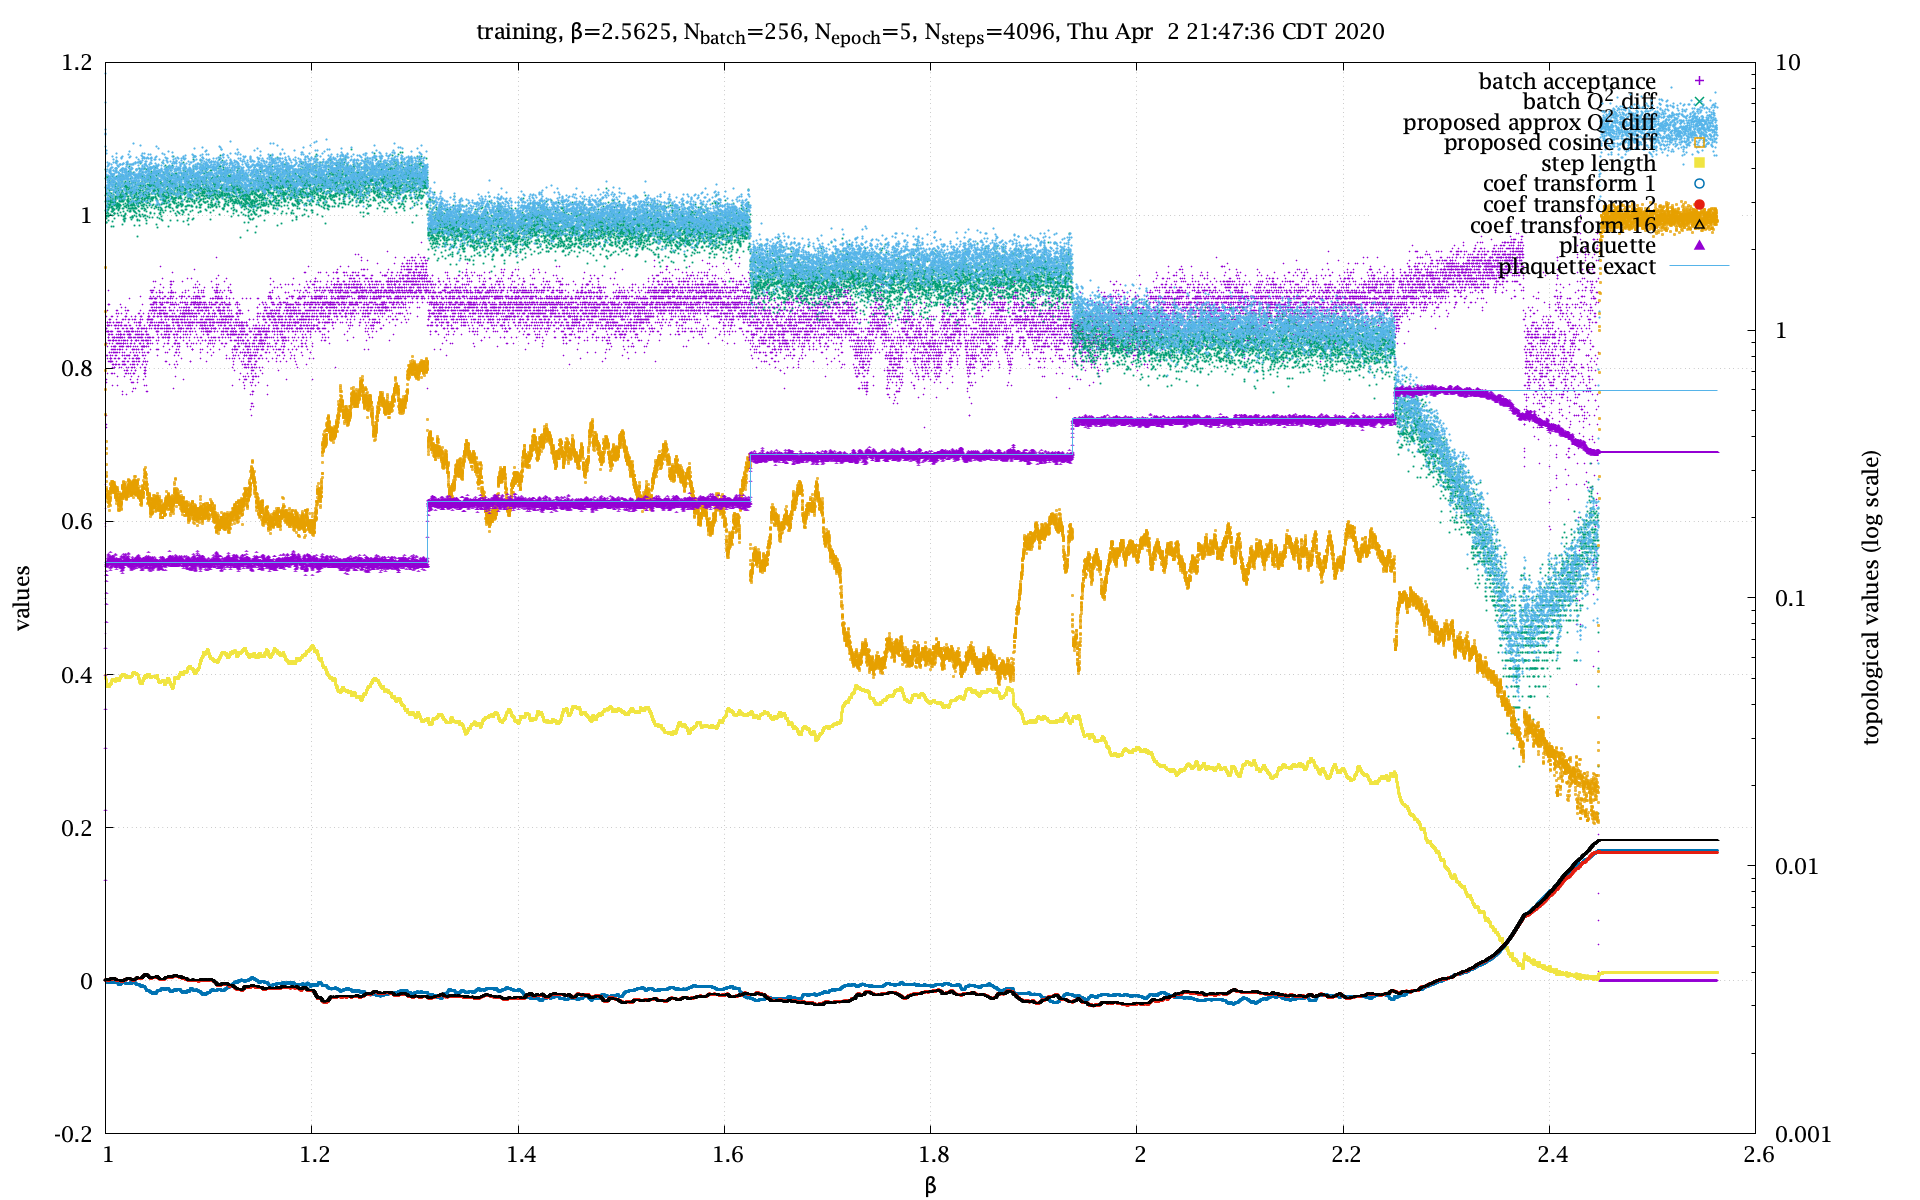
\includegraphics[width=\textwidth]{../../u1_2d/t2.png}
	\caption{\label{training-2}Annealed training steps for $V=8×8$ with 10 leapfrog steps.}
\end{figure}

\begin{figure}
	\centering
	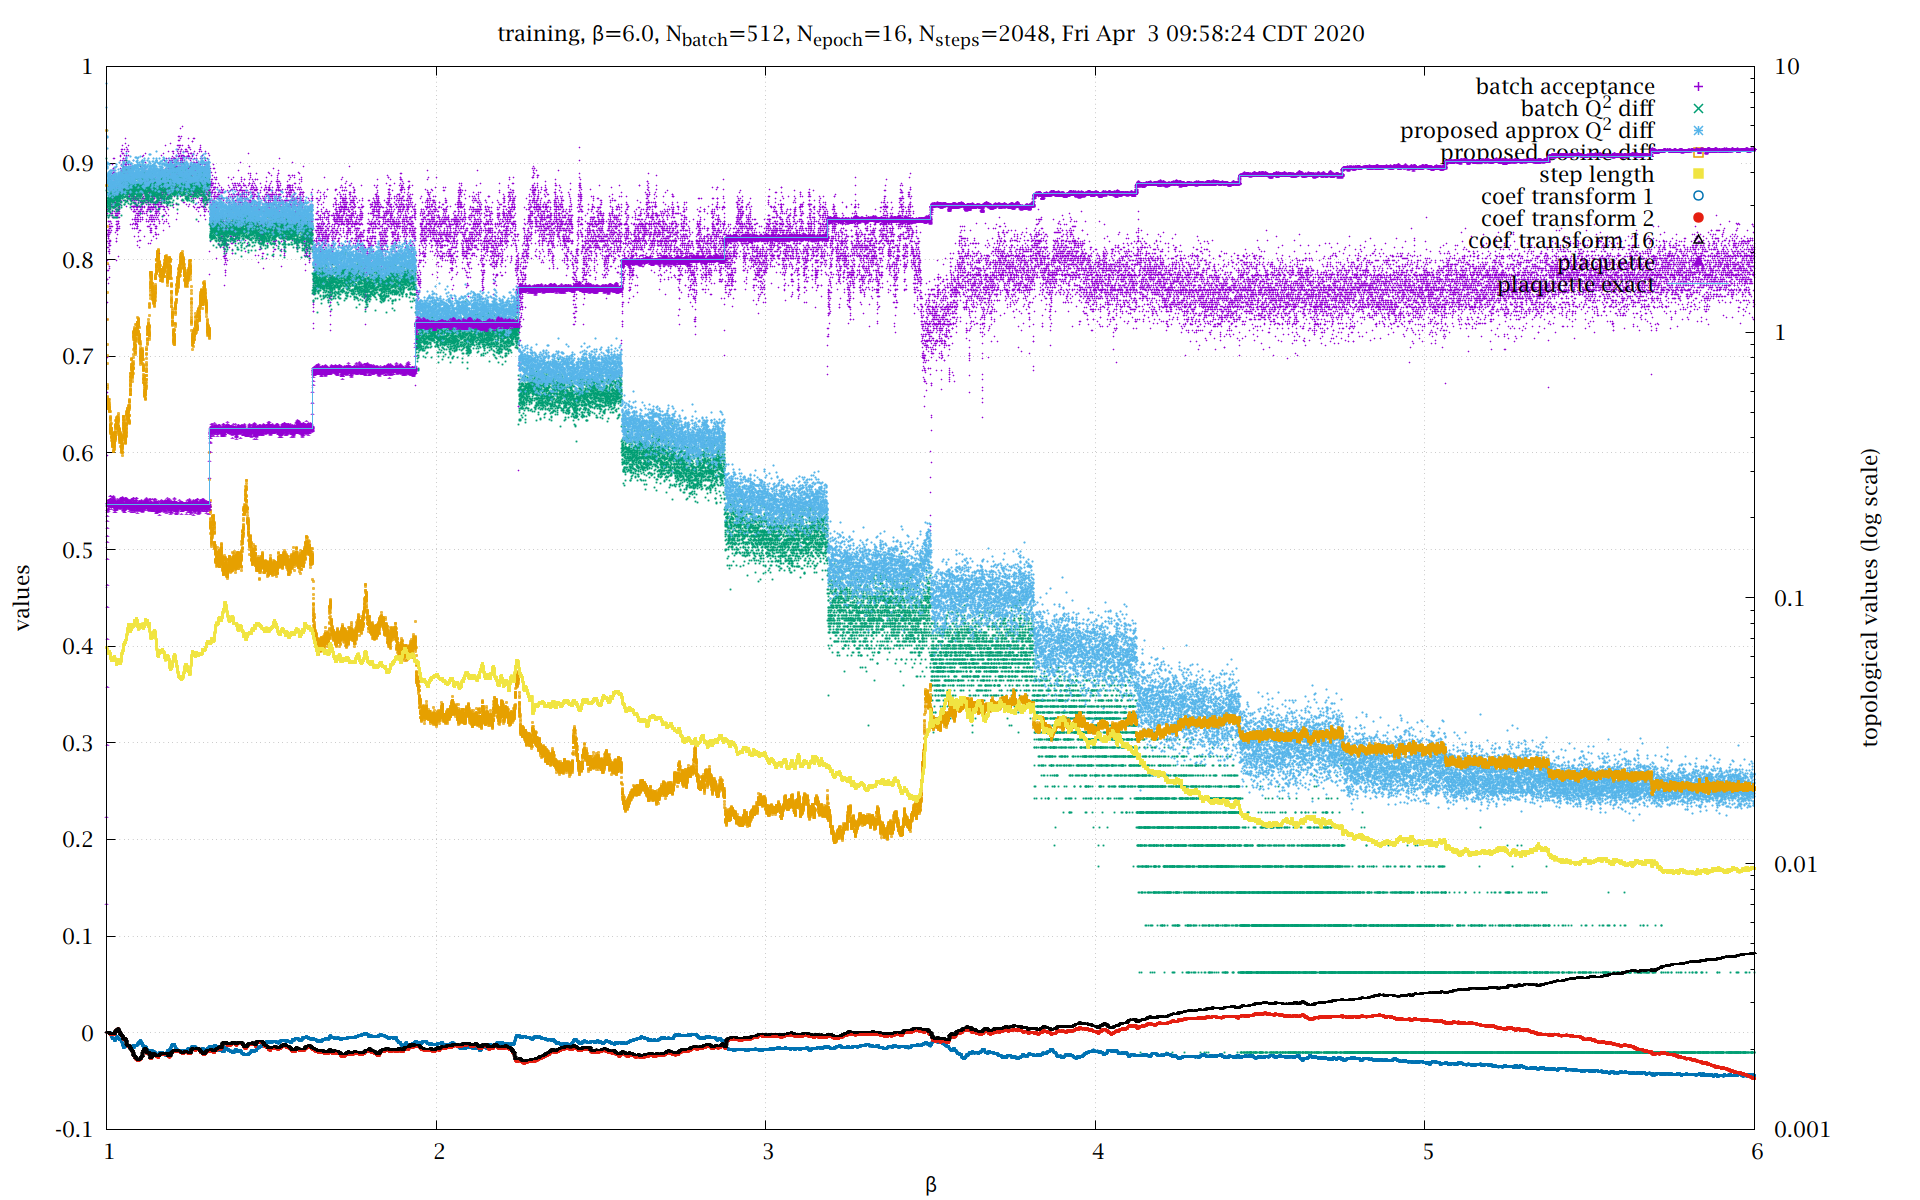
\includegraphics[width=\textwidth]{../../u1_2d/t5.png}
	\caption{\label{training-5}Annealed training steps for $V=8×8$ with 10 leapfrog steps.}
\end{figure}


\section{Discussions and plans}
\label{sec:discuss-plans}
A chain of ``stout smearing'' works for 1D.
Parameters trained for a chain of size 64 works for a chain of size 256.

Plans: Try optimize the trivializing map directly.
Test with 2D U(1) model.
Try neural network parametrized smearing.


\ifdefined\directlua
  \printbibliography
\else
  \bibliographystyle{JHEP}
  \bibliography{ref}
\fi

\end{document}
